\documentclass[margin=5mm]{standalone}
\usepackage{tikz}
\usepackage{array}
\usepackage{amssymb}
\usetikzlibrary{positioning, arrows.meta, calc, shapes.geometric}

\begin{document}
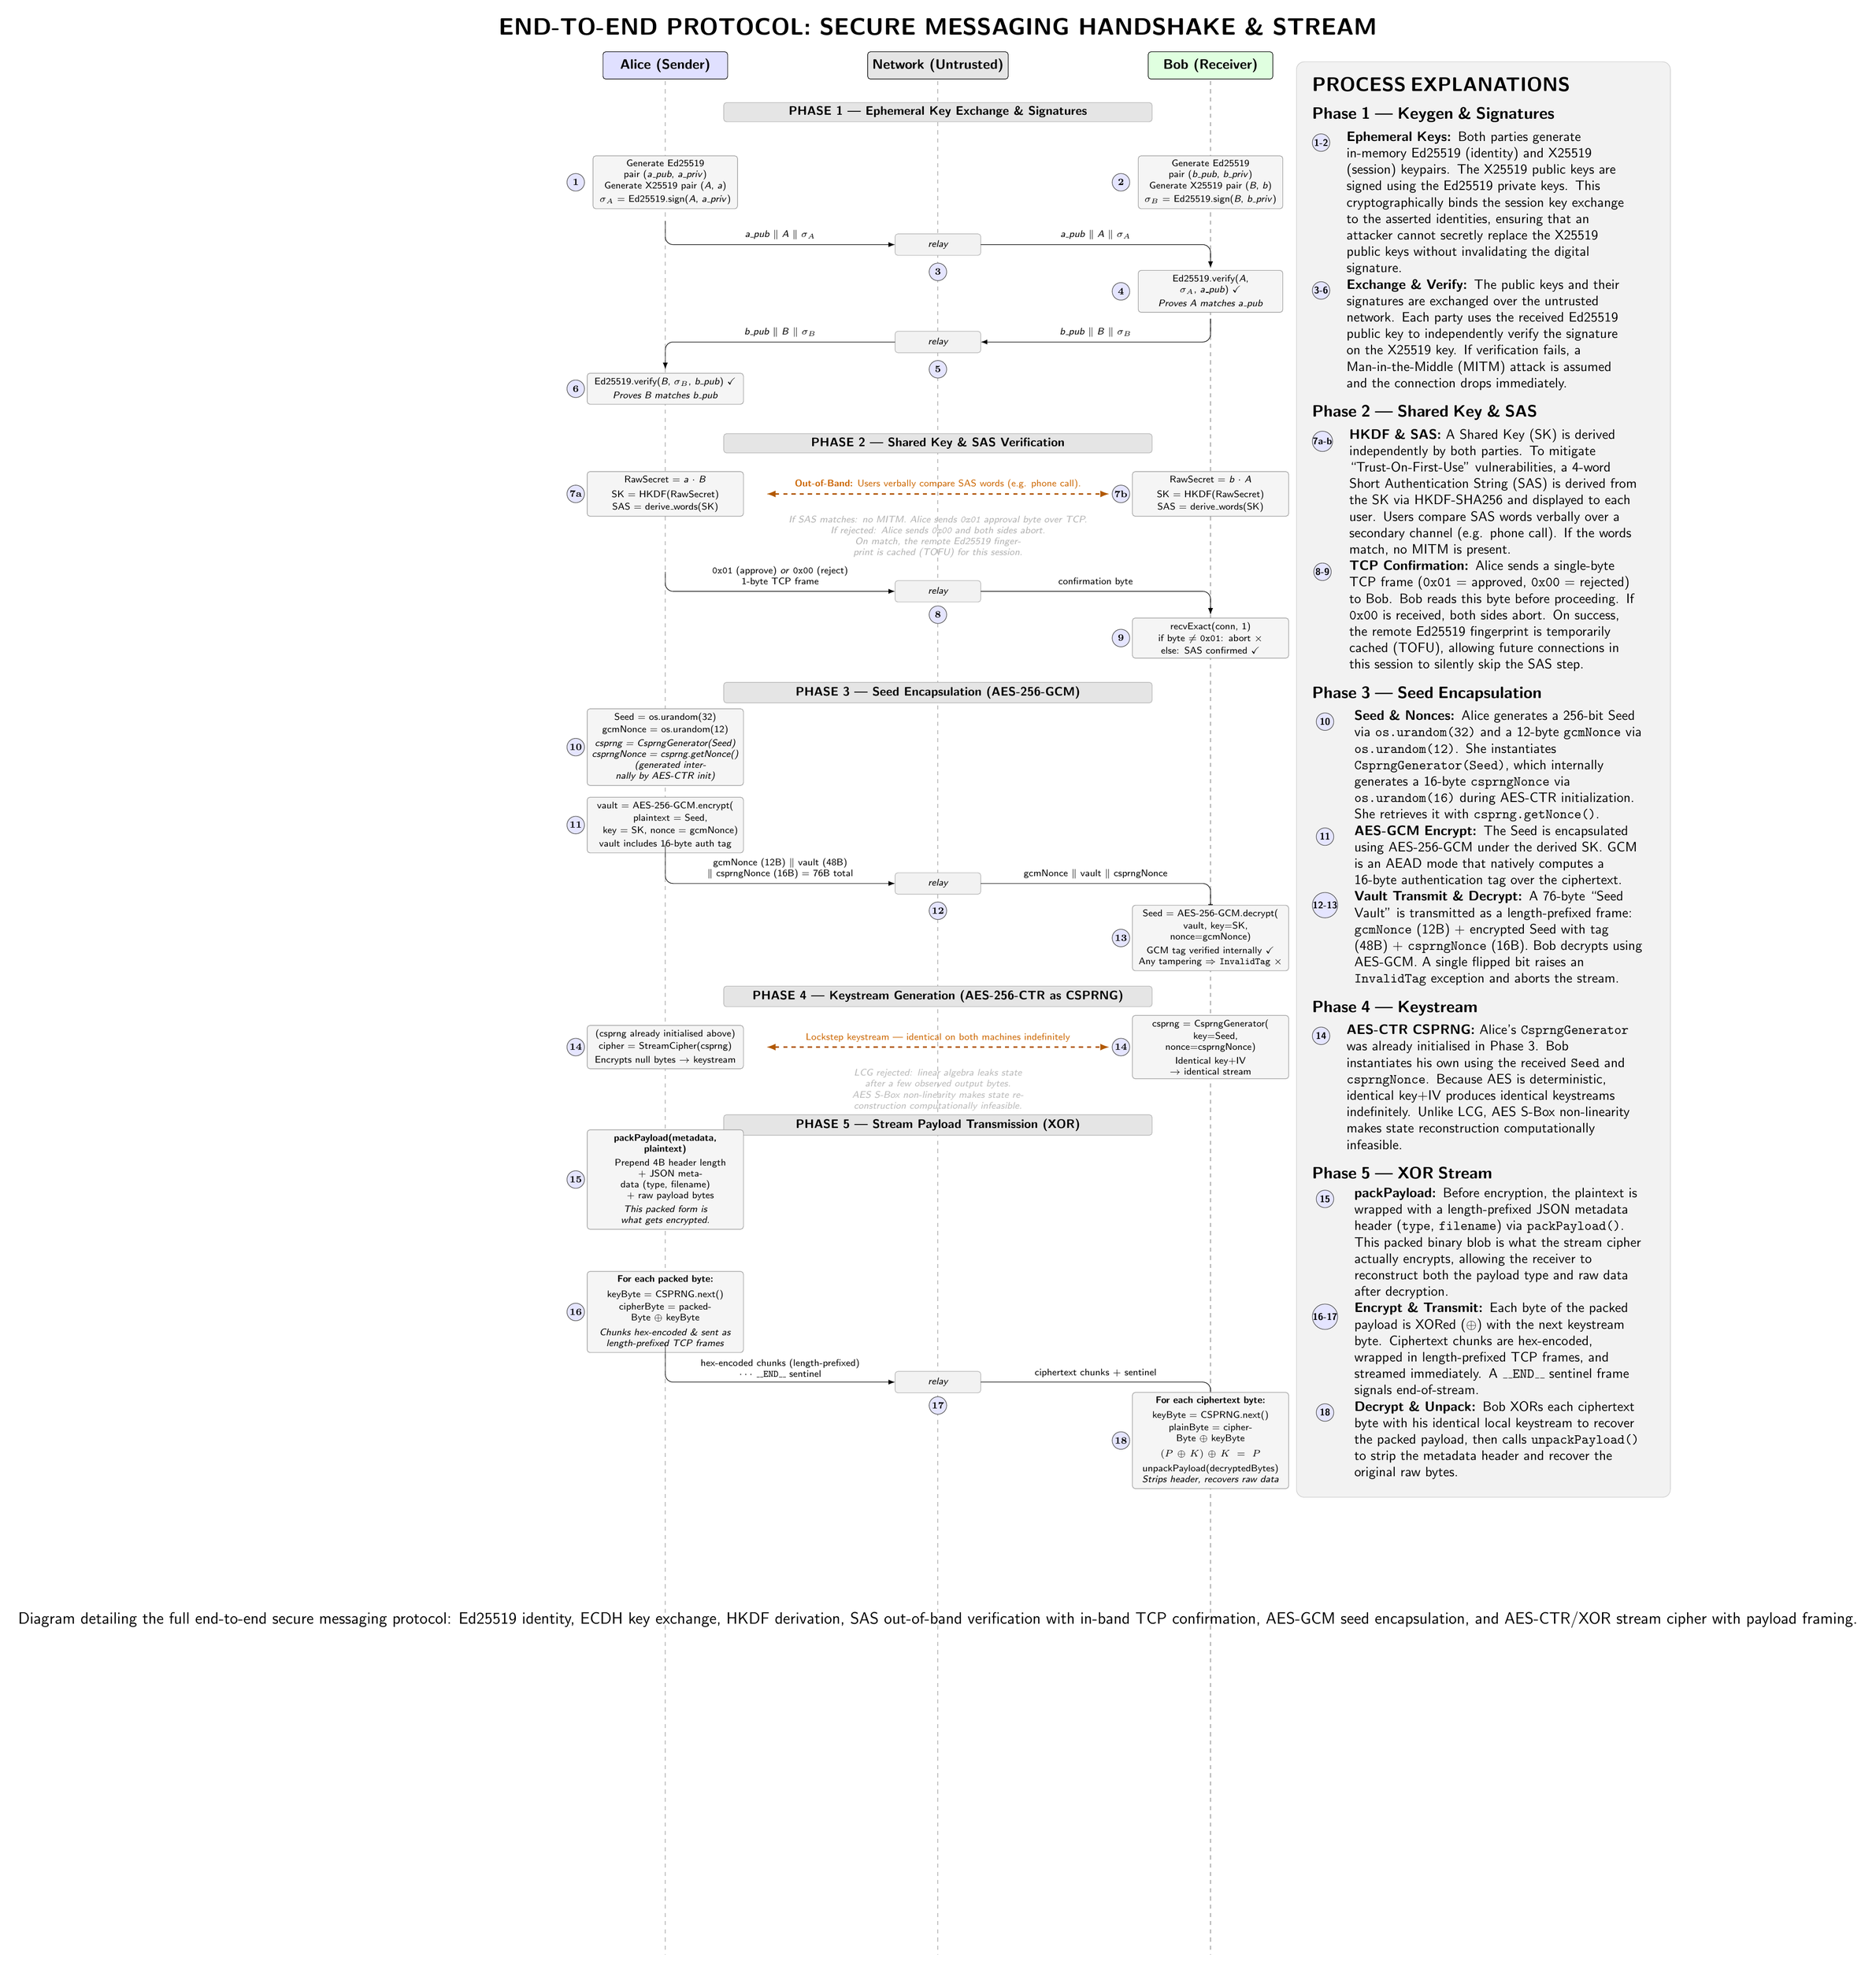
\begin{tikzpicture}[
    >=Latex,
    font=\sffamily,
    actor/.style={draw, fill=black!8, rounded corners=2pt,
                  minimum width=3.2cm, minimum height=0.7cm,
                  align=center, font=\bfseries\sffamily},
    compute/.style={draw=black!40, fill=black!4, rounded corners=2pt,
                    minimum width=3.2cm, align=center,
                    font=\scriptsize\sffamily, inner sep=3pt},
    phase/.style={fill=black!10, draw=black!30, rounded corners=2pt,
                  inner sep=3pt, font=\small\bfseries\sffamily, align=center},
    indicator/.style={circle, draw=black!70, fill=blue!10, inner sep=0pt,
                      minimum size=4.5mm, font=\scriptsize\bfseries, align=center},
    netbox/.style={draw=gray!60, fill=gray!10, rounded corners=2pt,
                   minimum width=2.2cm, minimum height=0.55cm,
                   align=center, font=\scriptsize\itshape\sffamily},
    msglabel/.style={font=\scriptsize\sffamily, align=center},
]

\def\xA{0}
\def\xN{7}
\def\xB{14}

% ============================================================
%  TITLE
% ============================================================
\node[font=\LARGE\bfseries\sffamily, anchor=center] at (7, 1.5)
    {END-TO-END PROTOCOL: SECURE MESSAGING HANDSHAKE \& STREAM};

% ============================================================
%  ACTOR HEADERS
% ============================================================
\node[actor, fill=blue!12]  at (\xA, 0.5) {Alice (Sender)};
\node[actor, fill=gray!20]  at (\xN, 0.5) {Network (Untrusted)};
\node[actor, fill=green!12] at (\xB, 0.5) {Bob (Receiver)};

\draw[dashed, gray!50, thick] (\xA, 0.1)  -- (\xA, -48);
\draw[dashed, gray!50, thick] (\xN, 0.1)  -- (\xN, -48);
\draw[dashed, gray!50, thick] (\xB, 0.1)  -- (\xB, -48);

% ============================================================
%  PHASE 1
% ============================================================
\node[phase, minimum width=11cm] at (7, -0.7)
    {PHASE 1 --- Ephemeral Key Exchange \& Signatures};

\node[compute, text width=3.5cm] at (\xA, -2.5)
    {Generate Ed25519 pair (\textit{a\_pub}, \textit{a\_priv})\\
     Generate X25519 pair (\textit{A}, \textit{a})\\[2pt]
     $\sigma_A$ = Ed25519.sign(\textit{A}, \textit{a\_priv})};
\node[indicator] at (\xA-2.3, -2.5) {1};

\node[compute, text width=3.5cm] at (\xB, -2.5)
    {Generate Ed25519 pair (\textit{b\_pub}, \textit{b\_priv})\\
     Generate X25519 pair (\textit{B}, \textit{b})\\[2pt]
     $\sigma_B$ = Ed25519.sign(\textit{B}, \textit{b\_priv})};
\node[indicator] at (\xB-2.3, -2.5) {2};

\draw[->, rounded corners=2mm] (\xA, -3.5) |- (\xN-1.1, -4.1);
\node[msglabel, above] at ($(\xA, -4.1)!0.5!(\xN-1.1, -4.1)$) {\textit{a\_pub} $\parallel$ \textit{A} $\parallel$ $\sigma_A$};
\node[netbox] at (\xN, -4.1) {relay};
\draw[->, rounded corners=2mm] (\xN+1.1, -4.1) -| (\xB, -4.7);
\node[msglabel, above] at ($(\xN+1.1, -4.1)!0.5!(\xB, -4.1)$) {\textit{a\_pub} $\parallel$ \textit{A} $\parallel$ $\sigma_A$};
\node[indicator] at (\xN, -4.8) {3};

\node[compute, text width=3.5cm] at (\xB, -5.3)
    {Ed25519.verify(\textit{A}, $\sigma_A$, \textit{a\_pub}) $\checkmark$\\[2pt]
     \textit{Proves A matches a\_pub}};
\node[indicator] at (\xB-2.3, -5.3) {4};

\draw[->, rounded corners=2mm] (\xB, -6.0) |- (\xN+1.1, -6.6);
\node[msglabel, above] at ($(\xB, -6.6)!0.5!(\xN+1.1, -6.6)$) {\textit{b\_pub} $\parallel$ \textit{B} $\parallel$ $\sigma_B$};
\node[netbox] at (\xN, -6.6) {relay};
\draw[->, rounded corners=2mm] (\xN-1.1, -6.6) -| (\xA, -7.3);
\node[msglabel, above] at ($(\xN-1.1, -6.6)!0.5!(\xA, -6.6)$) {\textit{b\_pub} $\parallel$ \textit{B} $\parallel$ $\sigma_B$};
\node[indicator] at (\xN, -7.3) {5};

\node[compute, text width=3.8cm] at (\xA, -7.8)
    {Ed25519.verify(\textit{B}, $\sigma_B$, \textit{b\_pub}) $\checkmark$\\[2pt]
     \textit{Proves B matches b\_pub}};
\node[indicator] at (\xA-2.3, -7.8) {6};

% ============================================================
%  PHASE 2
% ============================================================
\node[phase, minimum width=11cm] at (7, -9.2)
    {PHASE 2 --- Shared Key \& SAS Verification};

\node[compute, text width=3.8cm] at (\xA, -10.5)
    {RawSecret = \textit{a} $\cdot$ \textit{B}\\[3pt]
     SK = HKDF(RawSecret)\\[1pt]
     SAS = derive\_words(SK)};
\node[indicator] at (\xA-2.3, -10.5) {7a};

\node[compute, text width=3.8cm] at (\xB, -10.5)
    {RawSecret = \textit{b} $\cdot$ \textit{A}\\[3pt]
     SK = HKDF(RawSecret)\\[1pt]
     SAS = derive\_words(SK)};
\node[indicator] at (\xB-2.3, -10.5) {7b};

% Out-of-band SAS comparison (no network relay — bypasses the untrusted channel)
\draw[<->, thick, orange!70!black, dashed]
    (\xA+2.6, -10.5) -- (\xB-2.6, -10.5)
    node[midway, above, msglabel, text=orange!80!black]
    {\textbf{Out-of-Band:} Users verbally compare SAS words (e.g. phone call).};

\node[msglabel, text=gray!60, text width=8cm, align=center] at (7, -11.6)
    {\textit{If SAS matches: no MITM. Alice sends \texttt{0x01} approval byte over TCP.}\\
     \textit{If rejected: Alice sends \texttt{0x00} and both sides abort.}\\
     \textit{On match, the remote Ed25519 fingerprint is cached (TOFU) for this session.}};

% SAS confirmation byte: Alice -> Network -> Bob (in-band TCP)
\draw[->, rounded corners=2mm] (\xA, -12.5) |- (\xN-1.1, -13.0);
\node[msglabel, above, text width=5cm, align=center] at ($(\xA, -13.0)!0.5!(\xN-1.1, -13.0)$)
    {\texttt{0x01} (approve) \textit{or} \texttt{0x00} (reject)\\ 1-byte TCP frame};
\node[netbox] at (\xN, -13.0) {relay};
\draw[->, rounded corners=2mm] (\xN+1.1, -13.0) -| (\xB, -13.6);
\node[msglabel, above] at ($(\xN+1.1, -13.0)!0.5!(\xB, -13.0)$)
    {confirmation byte};
\node[indicator] at (\xN, -13.6) {8};

\node[compute, text width=3.8cm] at (\xB, -14.2)
    {recvExact(conn, 1)\\[1pt]
     if byte $\neq$ \texttt{0x01}: abort $\times$\\[1pt]
     else: SAS confirmed $\checkmark$};
\node[indicator] at (\xB-2.3, -14.2) {9};

% ============================================================
%  PHASE 3
% ============================================================
\node[phase, minimum width=11cm] at (7, -15.6)
    {PHASE 3 --- Seed Encapsulation (AES-256-GCM)};

\node[compute, text width=3.8cm] at (\xA, -17.0)
    {Seed     = os.urandom(32)\\[1pt]
     gcmNonce = os.urandom(12)\\[2pt]
     \textit{csprng = CsprngGenerator(Seed)}\\
     \textit{csprngNonce = csprng.getNonce()}\\
     \quad\textit{(generated internally by AES-CTR init)}};
\node[indicator] at (\xA-2.3, -17.0) {10};

\node[compute, text width=3.8cm] at (\xA, -19.0)
    {vault = AES-256-GCM.encrypt(\\[1pt]
     \quad plaintext = Seed,\\[1pt]
     \quad key = SK, nonce = gcmNonce)\\[2pt]
     vault includes 16-byte auth tag};
\node[indicator] at (\xA-2.3, -19.0) {11};

\draw[->, rounded corners=2mm] (\xA, -19.5) |- (\xN-1.1, -20.5);
\node[msglabel, above, text width=5cm, align=center] at ($(\xA, -20.5)!0.5!(\xN-1.1, -20.5)$)
    {gcmNonce (12B) $\parallel$ vault (48B)\\ $\parallel$ csprngNonce (16B) = 76B total};
\node[netbox] at (\xN, -20.5) {relay};
\draw[->, rounded corners=2mm] (\xN+1.1, -20.5) -| (\xB, -21.2);
\node[msglabel, above] at ($(\xN+1.1, -20.5)!0.5!(\xB, -20.5)$)
    {gcmNonce $\parallel$ vault $\parallel$ csprngNonce};
\node[indicator] at (\xN, -21.2) {12};

\node[compute, text width=3.8cm] at (\xB, -21.9)
    {Seed = AES-256-GCM.decrypt(\\[1pt]
     \quad vault, key=SK, nonce=gcmNonce)\\[2pt]
     GCM tag verified internally $\checkmark$\\
     Any tampering $\Rightarrow$ \texttt{InvalidTag} $\times$};
\node[indicator] at (\xB-2.3, -21.9) {13};

% ============================================================
%  PHASE 4
% ============================================================
\node[phase, minimum width=11cm] at (7, -23.4)
    {PHASE 4 --- Keystream Generation (AES-256-CTR as CSPRNG)};

\node[compute, text width=3.8cm] at (\xA, -24.7)
    {(csprng already initialised above)\\[1pt]
     cipher = StreamCipher(csprng)\\[2pt]
     Encrypts null bytes $\to$ keystream};
\node[indicator] at (\xA-2.3, -24.7) {14};

\node[compute, text width=3.8cm] at (\xB, -24.7)
    {csprng = CsprngGenerator(\\[1pt]
     \quad key=Seed, nonce=csprngNonce)\\[2pt]
     Identical key+IV $\to$ identical stream};
\node[indicator] at (\xB-2.3, -24.7) {14};

\draw[<->, thick, orange!70!black, dashed]
    (\xA+2.6, -24.7) -- (\xB-2.6, -24.7)
    node[midway, above, msglabel, text=orange!80!black]
    {Lockstep keystream --- identical on both machines indefinitely};

\node[msglabel, text=gray!55, text width=6.5cm, align=center] at (7, -25.8)
    {\textit{LCG rejected: linear algebra leaks state after a few observed output bytes.}\\
     \textit{AES S-Box non-linearity makes state reconstruction computationally infeasible.}};

% ============================================================
%  PHASE 5
% ============================================================
\node[phase, minimum width=11cm] at (7, -26.7)
    {PHASE 5 --- Stream Payload Transmission (XOR)};

\node[compute, text width=3.8cm] at (\xA, -28.1)
    {\textbf{packPayload(metadata, plaintext)}\\[2pt]
     \quad Prepend 4B header length\\
     \quad + JSON metadata (type, filename)\\
     \quad + raw payload bytes\\[2pt]
     \textit{This packed form is what gets encrypted.}};
\node[indicator] at (\xA-2.3, -28.1) {15};

\node[compute, text width=3.8cm] at (\xA, -31.5)
    {\textbf{For each packed byte:}\\[3pt]
     keyByte    = CSPRNG.next()\\[1pt]
     cipherByte = packedByte $\oplus$ keyByte\\[3pt]
     \textit{Chunks hex-encoded \& sent as}\\
     \textit{length-prefixed TCP frames}};
\node[indicator] at (\xA-2.3, -31.5) {16};

\draw[->, rounded corners=2mm] (\xA, -32.3) |- (\xN-1.1, -33.3);
\node[msglabel, above, text width=5cm, align=center] at ($(\xA, -33.3)!0.5!(\xN-1.1, -33.3)$)
    {hex-encoded chunks (length-prefixed)\\$\cdots$ \texttt{\_\_END\_\_} sentinel};
\node[netbox] at (\xN, -33.3) {relay};
\draw[->, rounded corners=2mm] (\xN+1.1, -33.3) -| (\xB, -34.1);
\node[msglabel, above] at ($(\xN+1.1, -33.3)!0.5!(\xB, -33.3)$)
    {ciphertext chunks $+$ sentinel};
\node[indicator] at (\xN, -33.9) {17};

\node[compute, text width=3.8cm] at (\xB, -34.8)
    {\textbf{For each ciphertext byte:}\\[3pt]
     keyByte   = CSPRNG.next()\\[1pt]
     plainByte = cipherByte $\oplus$ keyByte\\[3pt]
     $(P \oplus K) \oplus K = P$\\[3pt]
     unpackPayload(decryptedBytes)\\
     \textit{Strips header, recovers raw data}};
\node[indicator] at (\xB-2.3, -34.8) {18};

% ============================================================
%  EXPLANATORY SIDE PANEL
% ============================================================
\node[anchor=north west, fill=black!5, draw=black!20, rounded corners=2mm,
      inner sep=4mm, text width=8.8cm, align=left] at (16.2, 0.6) {
    \textbf{\Large PROCESS EXPLANATIONS}\\[3mm]

    \textbf{\large Phase 1 --- Keygen \& Signatures}\\[1.5mm]
    \begin{tabular}{@{}c >{\raggedright\arraybackslash}p{7.4cm}@{}}
        \tikz[baseline=-0.8ex]{\node[indicator]{1-2};}  &
        \textbf{Ephemeral Keys:} Both parties generate in-memory Ed25519 (identity) and X25519 (session) keypairs. The X25519 public keys are signed using the Ed25519 private keys. This cryptographically binds the session key exchange to the asserted identities, ensuring that an attacker cannot secretly replace the X25519 public keys without invalidating the digital signature.\\[1.5mm]
        \tikz[baseline=-0.8ex]{\node[indicator]{3-6};}  &
        \textbf{Exchange \& Verify:} The public keys and their signatures are exchanged over the untrusted network. Each party uses the received Ed25519 public key to independently verify the signature on the X25519 key. If verification fails, a Man-in-the-Middle (MITM) attack is assumed and the connection drops immediately.\\[1.5mm]
    \end{tabular}\\[3mm]

    \textbf{\large Phase 2 --- Shared Key \& SAS}\\[1.5mm]
    \begin{tabular}{@{}c >{\raggedright\arraybackslash}p{7.4cm}@{}}
        \tikz[baseline=-0.8ex]{\node[indicator]{7a-b};}  &
        \textbf{HKDF \& SAS:} A Shared Key (SK) is derived independently by both parties. To mitigate ``Trust-On-First-Use'' vulnerabilities, a 4-word Short Authentication String (SAS) is derived from the SK via HKDF-SHA256 and displayed to each user. Users compare SAS words verbally over a secondary channel (e.g. phone call). If the words match, no MITM is present.\\[1.5mm]
        \tikz[baseline=-0.8ex]{\node[indicator]{8-9};}  &
        \textbf{TCP Confirmation:} Alice sends a single-byte TCP frame (\texttt{0x01} = approved, \texttt{0x00} = rejected) to Bob. Bob reads this byte before proceeding. If \texttt{0x00} is received, both sides abort. On success, the remote Ed25519 fingerprint is temporarily cached (TOFU), allowing future connections in this session to silently skip the SAS step.\\[1.5mm]
    \end{tabular}\\[3mm]

    \textbf{\large Phase 3 --- Seed Encapsulation}\\[1.5mm]
    \begin{tabular}{@{}c >{\raggedright\arraybackslash}p{7.4cm}@{}}
        \tikz[baseline=-0.8ex]{\node[indicator]{10};} &
        \textbf{Seed \& Nonces:} Alice generates a 256-bit Seed via \texttt{os.urandom(32)} and a 12-byte \texttt{gcmNonce} via \texttt{os.urandom(12)}. She instantiates \texttt{CsprngGenerator(Seed)}, which internally generates a 16-byte \texttt{csprngNonce} via \texttt{os.urandom(16)} during AES-CTR initialization. She retrieves it with \texttt{csprng.getNonce()}.\\[1.5mm]
        \tikz[baseline=-0.8ex]{\node[indicator]{11};} &
        \textbf{AES-GCM Encrypt:} The Seed is encapsulated using AES-256-GCM under the derived SK. GCM is an AEAD mode that natively computes a 16-byte authentication tag over the ciphertext.\\[1.5mm]
        \tikz[baseline=-0.8ex]{\node[indicator]{12-13};} &
        \textbf{Vault Transmit \& Decrypt:} A 76-byte ``Seed Vault'' is transmitted as a length-prefixed frame: \texttt{gcmNonce} (12B) + encrypted Seed with tag (48B) + \texttt{csprngNonce} (16B). Bob decrypts using AES-GCM. A single flipped bit raises an \texttt{InvalidTag} exception and aborts the stream.\\[1.5mm]
    \end{tabular}\\[3mm]

    \textbf{\large Phase 4 --- Keystream}\\[1.5mm]
    \begin{tabular}{@{}c >{\raggedright\arraybackslash}p{7.4cm}@{}}
        \tikz[baseline=-0.8ex]{\node[indicator]{14};} &
        \textbf{AES-CTR CSPRNG:} Alice's \texttt{CsprngGenerator} was already initialised in Phase 3. Bob instantiates his own using the received \texttt{Seed} and \texttt{csprngNonce}. Because AES is deterministic, identical key+IV produces identical keystreams indefinitely. Unlike LCG, AES S-Box non-linearity makes state reconstruction computationally infeasible.\\[1.5mm]
    \end{tabular}\\[3mm]

    \textbf{\large Phase 5 --- XOR Stream}\\[1.5mm]
    \begin{tabular}{@{}c >{\raggedright\arraybackslash}p{7.4cm}@{}}
        \tikz[baseline=-0.8ex]{\node[indicator]{15};} &
        \textbf{packPayload:} Before encryption, the plaintext is wrapped with a length-prefixed JSON metadata header (\texttt{type}, \texttt{filename}) via \texttt{packPayload()}. This packed binary blob is what the stream cipher actually encrypts, allowing the receiver to reconstruct both the payload type and raw data after decryption.\\[1.5mm]
        \tikz[baseline=-0.8ex]{\node[indicator]{16-17};} &
        \textbf{Encrypt \& Transmit:} Each byte of the packed payload is XORed ($\oplus$) with the next keystream byte. Ciphertext chunks are hex-encoded, wrapped in length-prefixed TCP frames, and streamed immediately. A \texttt{\_\_END\_\_} sentinel frame signals end-of-stream.\\[1.5mm]
        \tikz[baseline=-0.8ex]{\node[indicator]{18};} &
        \textbf{Decrypt \& Unpack:} Bob XORs each ciphertext byte with his identical local keystream to recover the packed payload, then calls \texttt{unpackPayload()} to strip the metadata header and recover the original raw bytes.\\[1.5mm]
    \end{tabular}
};

% ============================================================
%  BOTTOM CAPTION
% ============================================================
\node[font=\large\sffamily, anchor=center] at (7, -39.4)
    {Diagram detailing the full end-to-end secure messaging protocol:
     Ed25519 identity, ECDH key exchange, HKDF derivation,
     SAS out-of-band verification with in-band TCP confirmation,
     AES-GCM seed encapsulation, and AES-CTR/XOR stream cipher with payload framing.};

\end{tikzpicture}
\end{document}
